\documentclass{article}
\usepackage[utf8]{inputenc}
\usepackage{amsmath,amssymb}
\usepackage{graphicx}
\usepackage[a4paper,margin=0.9cm]{geometry}
\usepackage{multicol}
\usepackage{sectsty}

\graphicspath{ {./img/} }

\DeclareMathOperator{\ima}{Im}
\newcommand\tab[1][0,5cm]{\hspace*{#1}}

\begin{document}
	\allsectionsfont{\small}
	\scriptsize
	
	\begin{multicols*}{3}
		\section{Assiomi}
		\textbf{Assiomi di kolmogorov:}	
		\begin{enumerate}
			\setlength\itemsep{0.1mm}
			\item Non negatività: \(P(A)>0\)
			\item Normalizzazione: \(P(\Omega)=1\)
			\item Additività: se ho 2 eventi disgiunti \(A\) e \(B\): (\(P(A\cap B)=0\)). Allora \(P(A\cup B)= P(A)+P(B)\)
		\end{enumerate}
		\subsection{Teorema delle probabilità totali:}
		Ho n eventi disgiunti: \(A_1,A_2,A_3...\)\\
		\[P(\bigcup_{i=1}^{n}A_i)= \sum_{i=1}^{n}P(A_i)\]\\
		Se \(P(A\cap B)\neq 0\) allora \(P(A\cup B)= P(A)+P(B)-P(A\cap B)\) (e varie combinazioni se ci sono più di 2 eventi analizzati)
		\subsection{Leggi di probabilità uniformi}
		\textbf{Legge uniforme discreta}\\	
		\(P(A)= \frac{\#\text{casi favorevoli ad}A}{\#\text{casi totali}} = \frac{|A|}{|\Omega|}\)\\
		\textbf{Legge uniforme continua}\\
		\(P(A)=\frac{\text{area}(A)}{\text{area}(\Omega)}\) \(\forall A\subseteq \Omega\)
		
		\section{Probabilità condizionate}
		\textbf{Definizione di probabilità condizionata:}
		\(P(A|B)=\frac{P(A\cap B)}{P(B)}\)\\
		Altra definizione di intersezione: \(P(A\cap B)= P(B)\cdot P(A|B) = P(A)\cdot P(B|A)\)\\\\
		\textbf{Regola moltiplicativa:}
		\(P(A\cap B \cap C)= P(A)\cdot P(B|A) \cdot P(C|A\cap B)\)\\
		\subsection{Teorema delle probabilità totali}
		Se ho \(A_1,A_2,A_3\) disgiunti che formano una partizione di \(\Omega\):\\
		\(P(B)= P(A_1)\cdot P(B|A_1)+ P(A_2)\cdot P(B|A_2)+ P(A_3)\cdot P(B|A_3)\)
		\subsection{Regola di Bayes}
		\[P(A|B)= \frac{P(B|A)\cdot P(A))}{P(B)}\]\\
		\textbf{Indipendenza}\\
		Se \(A \perp B\) allora \(P(B|A) = P(B) , P(A|B)= P(A)\)\\
		Due eventi si dicono indipendenti se: \(P(A\cap B)= P(A)\cdot P(B)\)
		\section{Calcolo combinatorio}
		\subsection{Permutazioni}
		In quanti modi posso ordinare questi n elementi distinti?\\
		casi tot \(=  n(n-1)(n-2)...=n!\)
		\subsection{Combinazioni}
		Calcolare il numero di sottoinsiemi con \(k\) elementi, partendo da un insieme con n elementi distinti. \(0\leq k \leq n\)\\
		\#sequenze ordinate di \(k\) elementi \(= \frac{n!}{(n-k)!k!}\)\\
		\(C_{n,k}= \binom{n}{k}\)\\\\
		\textbf{Probabilità binomiale}\\
		Date n prove indipendenti, probabilità di successo della singola prova \(P(\text{successo})= p\), la prob. di avere k successi su n prove è: \(p^k \cdot (1-p)^{n-k} \cdot \binom{n}{k}\)
		\subsection{Coefficiente multinomiale (partizioni)}
		Ho uno spazio di probabilità uniforme ed eseguo \(n\) prove indipendenti (es. estrazioni con reinserimento), voglio calcolare quante sequenze con \(k_i\) estrazioni di tipo \(i\) ci sono.\\
		\#totale di scelte \(= \frac{n!}{k_1!k_2!k_3!k_4!} = \binom{n}{k_1,k_2,k_3,k_4}\)
		
		\section{Variabili aleatorie discrete}
		
		
		
		
		
		
		\subsection{Valore atteso}
		\[E[X]= \sum_{x\in \mathbb{R}}^{} x \cdot p_x(x)\]
		Moltiplico sommo il prodotto di ogni realizzazione con il suo peso ovvero la sua probabilità.\\
		\textbf{Legge dello statistico inconsapevole}\\
		Data v.a. \(Y= g(X)\), \(Y\) è una v.a.\\
		\(E[Y]= E[g(x)]\)\\\\
		Nel caso lineare:\\
		\(E[\alpha X + \beta] = \alpha E[X] + \beta\)\\
		\textbf{Valore atteso condizionato}\\
		\(E[X|B]= \sum_{x\in \mathbb{R}}^{} x \cdot p_{X|B} (x) \)\\
		\textbf{Legge dell'aspettativa totale}\\
		Con \(A_1,A_2,...,A_n\) partizioni di \(\Omega\)\\
		\(E[X] = \sum_{i_1}^{n} P(A_1) \cdot E[X|A_i]\)
		
		\subsection{Varianza}
		\[Var[X] = E[(X-E[X])^2] = E[X^2]- E[X]^2\]
		La varianza è il momento di ordine 2.\\
		\textbf{Proprietà varianza}\\
		\(Var[X] \geq 0 \qquad \forall \ \text{v.a.} \ X\)\\
		\(Var[\alpha X + \beta] = \alpha^2 \cdot Var[X]\)\\
		\textbf{Scarto quadratico medio}\\
		\(\sigma = \sqrt{Var[X]}\)\\
		\section{V.a. discrete multiple}
		\subsection{Legge di probabilità congiunta}
		Ho 2 v.a. \(X\) e \(Y\), \(P({X=x}\cap{Y=y}) = p_{X,Y} (x,y) \)\\\\
		Per trovare la legge marginale di X: \(p_x (x) = \sum_{y}^{} p_{X,Y} (x,y)\)\\
		\textbf{Legge di probabilità condizionata}
		\(p_{X|Y} (x|y) = \frac{p_{X,Y} (x,y)}{\sum_{t}^{} p_{X,Y} (t,y)} = \frac{p_{X,Y} (x,y)}{p_Y (y)}\)\\
		\textbf{Regola moltiplicativa}\\
		\(p_{X,Y} (x,y) = p_{X|Y} (x|y) \cdot p_Y (y) = p_{Y|X} (y|x) \cdot p_X (x)\)\\
		\subsection{Variabili aleatorie indipendenti}
		Due v.a. \(X\) e \(Y\) sono dette indipendenti \((X\perp Y)\) \(\iff\) \(p_{X,Y} (x,y) = p_X (x)\cdot p_Y (y) \)\\
		
		\subsection{Valore atteso per v.a. multiple}
		Statistica congiunta di \(X\) e \(Y\).\\
		\(E[g(X,Y)] = \sum_{x}^{}\sum_{y}^{} g(x,y) \cdot p_{X,Y} (x,y)\)\\
		Caso lineare: \(E[\alpha X + \beta Y + \gamma] = \alpha E[X] + \beta E[Y] + \gamma\) \\
		Se \(X \perp Y\) allora \(E[X \cdot Y] = E[X] \cdot E[Y]\)
		
		\subsection{Varianza per v.a. multiple}
		\(Var[X+Y]= Var[X] + Var[Y] +2(E[XY] -E[X]E[Y])\)\\
		Se \(X\perp Y\) allora \(Var[X+Y] = Var[X] + Var[Y]\)\\
		
		\section{Variabili aleatorie continue}
		\textbf{Valore atteso e varianza}\\
		\(E[X] = \int_{\mathbb{R}}^{} x \cdot f_x (x) dx\)\\
		Legge dello statistico inconsapevole: \(E[g(X)] = \int_{\mathbb{R}}^{} g(x) \cdot f_x (x) dx\)\\
		\(Var[X] = E[X^2] - E[X]^2\)
		
		
		
		\subsection{Funzione cumulativa di probabilità}
		\(P(X\leq x) = F_x (x) = \int_{-\infty}^{x} f_x (t) dt\)\\
		\textbf{Proprietà}
		\begin{itemize}
			\item \(0\leq F_x (x) \leq 1\)
			\item \(F_x\) è una funzione non decrescente \(\forall x \in \mathbb{R}\)
			\item \(\frac{d}{dx} F_x (x) = f_x (x)\), \(F_x\) è la funzione integrale di \(f_x\)  
		\end{itemize}
				
		\section{V.a. continue multiple}
		\textbf{Densità di probabilità congiunta}\\
		\(P((X,Y)\in S) = \iint_{(x,y)\in S}f_{X,Y} (x,y) dxdy \)\\ \(f_{X,Y} \) è la densità di probabilità congiunta.\\
		\textbf{Valore atteso}\\
		\(E[g(X,Y)] = \iint_{\mathbb{R}} g(x,y)\cdot f_{X,Y}(x,y) dxdy\) \\Con g funzione deterministica nota.\\
		\textbf{Legge di probabilità marginale}\\
		\(f_x(x) = \int_{\mathbb{R}}^{} f_{X,Y}(x,y) dy\)\\
		Densità marginale di X.\\
		\textbf{Indipendenza tra due v.a. continue}\\
		\(X\) e \(Y\) sono dette indipendenti \(\iff\) \(f_{X,Y}(x,y) = f_X(x)\cdot f_Y(y) \qquad \forall (x,y) \in \mathbb{R}^2\)\\
		\textbf{Densità di probabilità condizionata}\\
		\(f_{Y|X}(y|x) = \frac{f_{X|Y} (x,y)}{f_X (x)} = \frac{f_{X,Y} (x,y)}{\int_{\mathbb{R}} f_{X,Y} (x,t) dt}\)\\
		
		
		\section{Regola di bayes e funzioni di v.a.}
		\textbf{Regola di bayes nel continuo}\\
		\(f_{X|Y} (x|y) = \frac{f_{Y|X} (y|x)\cdot f_X(x)}{f_Y (y)}\)\\
		Per le v.a. discrete basta cambiare la funzione continua con la probabilità.\\
		\subsection{Calcolo della funzione di una v.a. continua}
		Ho \(X\) v.a. con legge nota \(f_x\) e \(Y=g(X)\) con \(g\) deterministica e nota, voglio trovare \(f_y\).\\
		\textbf{Approccio tramite la cumulata}\\
		1- Calcolo la cumulata di \(Y\).\\
		\(F_Y(y) = P(Y\leq y)\)\\
		2. Calcolo \(f_Y\)\\
		\(f_Y (y)= \frac{d}{dy} F_Y (y)\)\\\\
		\textbf{Trasformazioni lineari di v.a.}\\
		\(X\) è una v.a. con legge \(f_X\) nota e \(Y = aX + b\) con costanti note.\\
		\(f_Y(y) = f_x(\frac{y-b}{a}\cdot \frac{1}{|a|})\), se \(a=0\) allora \(Y=b\)\\
		\textbf{Trasformazione monotona di v.a.}\\
		\(Y = g(X) \) con \(g\) deterministica nota e strettamente monotona.\\
		\(f_Y (y) = \frac{f_X (x) }{|\frac{dg}{dx} (x)|} = \frac{f_X (g^{-1} (y))}{|\frac{dg}{dx} (g^{-1} (y))|}\)\\
		Con \(y= g(x)\) e \(x=g^{-1}(y)\)\\
		Nota: se \(g\) non è strettamente monotona (ad es. \(g(x)= x^2\)) la \(f_Y(y) \) sarà: "formula diretta con \(g\) decrescente" + "formula diretta con \(g\) crescente".\\
		\section{Statistiche congiunte}
		\textbf{Legge della somma di v.a.}\\
		Date \(X\) e \(Y\) due v.a. discrete e \(X \perp Y\) e \(W = X+Y\)\\
		\(P_W(w) = P(W=w) = P(X+Y = w) = \sum_x p_X (x) \cdot p_Y (w-x)\), \(\qquad y=w-x\)\\
		La legge della somma di due v.a. \textbf{indipendenti} è la convoluzione delle leggi di probabilità.\\
		\textbf{Calcolo della somma di convoluzione con il metodo grafico}\\
		- Sovrapporre graficamente le 2 leggi di prob\\
		- "Ribaltare" una delle 2 leggi (ad es. \(P_Y\))\\
		- Traslare di \(w\) posizioni la legge che ho ribaltato (traslazione a destra se \(w > 0\))\\
		- Moltiplicare le prob. e sommare\\
		\textbf{Caso v.a. continue}\\
		\(W=X+Y\), \(\quad X\perp Y\), \(\quad X\) e \(Y\) sono v.a. continue.\\
		\(f_W(w) = \int_{-\infty}^{+ \infty} f_X (x) \cdot f_Y(w-x) dx \)\\
		Integrale di convoluzione\\
		\textbf{Somma di due gaussiane indipendenti}\\
		\(W=X+Y \), \(\quad X \sim N(\mu_x,\sigma^2_x)\),\(\quad Y \sim N(\mu_y,\sigma^2_y)\), \(\quad X\perp Y\)\\
		La forma di \(W\) è sempre gaussiana.\\
		\(E[W] =E[X+Y]= E[X] + E[Y]= \mu_x + \mu_y\)\\
		\(Var[W]= Var[X+Y] = Var[X]+Var[Y]= \sigma^2_x +\sigma^2_y\)\\
		\(f_W(w)= \frac{1}{\sqrt{2\pi (\sigma^2_x +\sigma^2_y)}}\cdot e^{\frac{w^2}{2(\sigma^2_x +\sigma^2_y)}}\)\\ (questa se \(\mu\) = 0)\\
		\subsection{Covarianza}
		\(Cov[X,Y] = E[XY] -E[X]E[Y]\)\\\\
		\textbf{Note:}\\
		- \(Cov[X,X] = Var[X]\)\\
		- Se \(E[X] = 0 \)o \(E[Y] = 0\) allora \(Cov[X,Y] = E[XY]\)\\
		- Se \(X\perp Y\) allora \(Cov[X,Y] =0\)\\
		- Se \(Cov[X,Y] = 0 \nRightarrow X\perp Y\)\\ 
		\textbf{Coefficiente di correlazione lineare}\\
		Versione adimensionale della covarianza.\\
		\(\rho[X,Y] = \frac{Cov[X,Y]}{\sigma_x\sigma_y}= E[\frac{(X-E[X])}{\sigma_x}\cdot \frac{(Y-E[Y])}{\sigma_y}]\)\\
		Proprietà:\\
		- \(0\leq|\rho[X,Y]| \leq 1\)\\
		In particolare se \(|\rho[X,Y]| = 1\) allora \(Y=aX+b\)\\
		- \(X\perp Y \implies\rho[X,Y] = 0 \)
		\section{Valore atteso e varianza condizionati}
		\textbf{Legge delle aspettazioni iterate}\\
		\(E[Y] = E[E[Y|X]]\)\\
		\textbf{Legge della variazione totale}\\
		\(Var[x] = E[Var[X|Y]] + Var[E[X|Y]] \)\\
		
		
		\section{Successioni variabili aleatorie}
		\subsection{Disuguaglianza di Markov}
		Se \(X > 0\) allora \(E[X] \geq a \cdot P(X\geq a) \qquad \forall a\geq 0\)\\\\
		\(P(X\geq a) \leq \frac{E[X]}{a}\)\\
		\subsection{Disuguaglianza di chebyshev}
		\(Var[X] \geq a \cdot P((X-E[X])^2 \geq a) \qquad \forall a\geq 0\)\\\\
		Con \(k= a^2\),\(\qquad P(|X-E[X]|\geq k) \leq \frac{Var[X]}{k^2}\)\\
		
		
		\subsection{Convergenza in probabilità}
		Data una successione di v.a. \(\{A_n\}\) e un numero \(a\), Si dice che \(\{A_n\}\) converge ad \(a\) se:\\
		\(\lim_{n \rightarrow \infty} P(|A_n - a| \geq \epsilon ) = 0 \qquad \forall \epsilon > 0\)\\\\
		\textbf{Test generale}\\
		\(\lim_{n \rightarrow \infty} P(|A_n - a| \geq \epsilon ) =\\ \lim_{n\rightarrow\infty}\int_{\epsilon}^{+\infty} f_{A_n}(x) dx\)\\
		Se questo valore fa 0, c'è convergenza.\\
		
		\textbf{Uso markov(o chebyshev nello stesso modo) per provare la convergenza in probabilità}\\
		Esempio com markov.\\
		\(\lim_{n \rightarrow \infty} P(|A_n - a| \geq \epsilon ) \leq \lim_{n \rightarrow\infty}\frac{E[X_n]}{a} \)\\\\
		Se \(\lim_{n \rightarrow\infty}E[X_n] = 0\) allora per forza converge ad a.\\
		
		\subsection{Media campionaria e legge dei grandi numeri}
		Date \(X_1,X_2,...,X_n\) v.a. i.i.d.\\
		Media campionaria: \(M_n= \frac{X_1+X_2+...+X_n}{n} \)\\ è una v.a.\\
		Dato che le varie v.a. sono i.i.d.\\ \(E[M_n] =E[X_1]=E[X]\)\\
		\(Var[M_n] = \frac{Var[X_1]}{n} \)\\ che con \(n \rightarrow \infty \qquad\) \(Var[M_n] \rightarrow 0\)\\\\
		\textbf{Legge (debole) dei grandi numeri}\\
		\(M_n \longrightarrow^P E[M_n] = E[X]\)\\
		
		\section{Teorema centrale del limite}
		CLT: Siano \(X_i\) v.a. i.i.d. con varianza finita \(\sigma^2\) sia\\
		\(Z_n =  \frac{X_1+X_2+...+X_n - n\mu}{\sqrt{n\sigma^2}} \) e sia \(Z\sim N(0,1)\), allora \(F_{Z_n}(c) \rightarrow^{n\rightarrow \infty} F_Z(c)=\Phi(c) \) per ogni c \(\in \mathbb{R}\)	
		
		\section{Processi di bernoulli}
		Def: una sequenza di prove (v.a.) di bernoulli i.i.d.\\
		\(X_i \sim Bern(p) \), ogni \(X_i\) è i.i.d.\\
		\textbf{Numero di successi S in n istanti temporali}\\
		S = numero di successi in n istanti\\
		\(S \sim Bin(n,p)\) \\
		\textbf{Tempi di interarrivo}\\
		\(T_1\) = numero di prove fino al primo arrivo\\
		\(T_1 \sim Geom(p)\)\\
		\(T_1\) gode di perdita di memoria\\
		\textbf{Tempo al k-esimo arrivo}\\
		\(P(Y_k = t) \sim \\ \left\{
		\begin{alignedat}{2}
			p^k\cdot (1-p)^{t-k}\cdot\binom{t-1}{k-1}  & \quad k=1,2,3,...\\
			0            & \quad \text{altrimenti}
		\end{alignedat}
		\right.\)\\
		\(E[Y_k] = \frac{k}{p}\), \(Var[Y_k]= k\frac{(1-p)}{p^2}\)\\
		\textbf{Splitting di un processo di bernoulli}\\
		Con \(q\) la prob che un arrivo vada nel processo \(P_1\)\\
		\(P_1 \sim BP(p\cdot q)\)\\
		\(P_1 \sim BP(p\cdot (1-q))\)\\
		\textbf{Merging di un processo di bernoulli}\\
		Con \(p\) e \(q\) le probabilità dei due BP\\
		\(P\sim BP(p+q-p\cdot q)\)\\
		\section{Processi di poisson}
		-Processo a tempo continuo (mantiene le stesse proprietà del processo di Bernoulli es. perdita di memoria)\\
		\textbf{Intensità media degli arrivi (per unità di tempo \(\tau\))}\\
		\(P(k,\tau) =\)costante\\
		\textbf{Distribuzione del numero di arrivi in un intervallo di tempo finito}\\
		\(P(N_{[0,\tau]} = k )= 
		\left\{
		\begin{alignedat}{2}
			\frac{(\lambda \tau )^k}{k!}e^{-\lambda\tau}  & \quad k=1,2,3,...\\
			0            & \quad \text{altrimenti}
		\end{alignedat}
		\right.\)\\\\
		Legge di Poisson: \(N_{[0,\tau]} \sim Poisson(\lambda\cdot\tau)\)\\
		\(E[N_{[0,\tau]}] = \lambda\tau \)\(\qquad Var[N_{[0,\tau]}] = \lambda\tau\)\\
		\textbf{Distribuzione del tempo al k-esimo arrivo}\\
		\(Y_k\): tempo al k-esimo arrivo\\
		\(f_{Y_k} = 
		\left\{
		\begin{alignedat}{2}
			\frac{(\lambda t)^{k-1}}{(k-1)!}e^{-\lambda t}\lambda  & \quad t\geq 0,k>1\\
			0            & \quad \text{altrimenti}
		\end{alignedat}
		\right.\)\\
		Legge di Erlang, \(Y_k \sim Erlang-k(\lambda)\)\\
		\(E[Y_k] = \frac{k}{\lambda}\)\\
		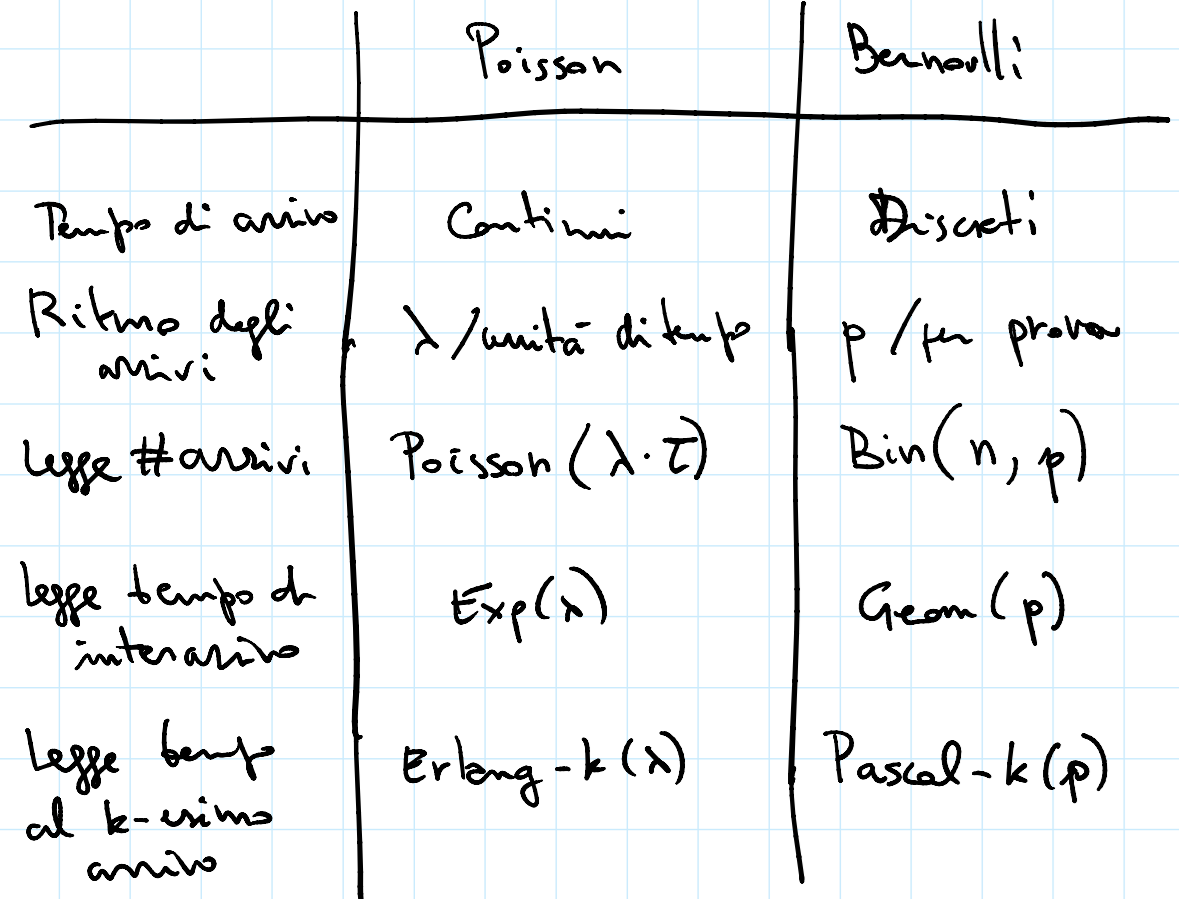
\includegraphics[scale=0.2]{pb}\\\\
		\textbf{Splitting e merging di un processo di Poisson}\\
		- Il processo generato dal merging di due PP indipendenti è un PP con itensità \(\lambda = \lambda_1 + \lambda_2\)\\
		- Il processo generato dallo split di un PP (Le "decisioni" di split devono essere tutte \(\perp\)) è \(PP_1(\lambda p)\) dove \(p\) è la probabilità di finire nel \(PP_1\)\\\\
		\textbf{Incidenza casuale per processi di Poisson}\\
		Con un \(PP\) iniziato da molto tempo la distribuzione della lunghezza dell'intervallo tra due arrivi è \(\sim Erlang-2(\lambda)\)\\
		(approssimazione della binomiale con poissoniana?)\\
		
		
		
		
		
		
		
		
		\section{Variabili aleatorie note}
		
		\subsection{V.a. uniforme continua}
		\(X \sim \mathbb{U}[a,b] \)\\
		\begin{equation*}
			f_x (x) \sim
			\left\{
			\begin{alignedat}{2}
				\frac{1}{b-a}  & \qquad a\leq x \leq b\\
				0            & \qquad \text{altrimenti}
			\end{alignedat}
			\right.
		\end{equation*}
		\(E[X] = \frac{a+b}{2}\), \(Var[X] = \frac{(b-a)^2}{12}\), \(\sigma_x = \frac{b-a}{\sqrt{12}}\)\\
		
		\subsection{V.a. gaussiana}
		\(X \sim Norm[E[x],Var[X]] = Norm[\mu,\sigma^2]\)\\
		\(F_x(x) = P(X\leq x) = \Phi(\frac{x-\mu}{\sigma})\)\\
		\(f_X(x)= \frac{1}{\sqrt{2\pi \sigma^2}}e^{-\frac{1}{2}(\frac{x-\mu}{\sigma})^2}\)\\
		\textbf{Combinazioni lineari di gaussiane}\\
		Se \(X_1,X_2,...X_n\) sono \(n\) v.a. gaussiane tra loro indipendenti con ciascuna valore atteso \(\mu_i\) e varianza \(\sigma^2_i\) allora la v.a. \(Y= \alpha_1X_1+\alpha_2X_2+...+\alpha_nX_n\) è una gaussiana con valore atteso \(\mu = \alpha_1\mu_1+\alpha_2\mu_2+...+\alpha_n\mu_n\) e varianza \(\sigma^2 = \alpha_1\sigma_1+ \alpha_2\sigma_2+...+\alpha_n\sigma_n\)
		
		
		\subsection{V.A. esponenziale}
		\(X\sim Exp[\lambda], \lambda > 0\)\\
		\(f_X(x) = \lambda e^{-\lambda x} \qquad \forall x>0\)\\
		\(F_X(x) = 1-e^{-\lambda x} \qquad \forall x>0\)\\
		\(E[X] = \frac{1}{\lambda}, Var[X] = \frac{1}{\lambda^2}\)\\
		\subsection{Variabile aleatoria geometrica}
		La v.a. geometrica risponde al problema: facendo esperimenti ripetuti, qual'è la probabilità di ottenere il primo successo alla k-esima prova.\\ 
		\begin{equation*}
			X \sim
			\left\{
			\begin{alignedat}{2}
				(1-p)^{k-1}  & \qquad k=1,2,3,...\\
				0            & \qquad \text{altrimenti}
			\end{alignedat}
			\right.
		\end{equation*}
		\(X \sim Geom(p)\) Dove \(p\) è la probabilità di successo nella singola prova.\\
		\(E[X] = \frac{1}{p}, Var[X] = \frac{1-p}{p^2}\)\\\\
		\textbf{Legge di perdita di memoria}\\
		\(p_{x-t|X>t}(k) = p_x (k) \implies E[X-t|X>t] = E[X]\) (Vale solo per v.a. \(Geom\) e \(Exp\))
		
		\subsection{Variabile aleatoria binomiale}
		La v.a. binomiale risponde al problema: facendo esperimenti ripetuti qual'è la probabilità di ottenere esattamente k successi?.\\ 
		\begin{equation*}
			X \sim
			\left\{
			\begin{alignedat}{2}
				\binom{n}{k}\cdot p^k \cdot (1-p)^{n-k}  & \qquad k=1,2,3,...\\
				0            & \qquad \text{altrimenti}
			\end{alignedat}
			\right.
		\end{equation*}
		\(X \sim Bin(n,p)\) Dove \(p\) è la probabilità di successo nella singola prova ed n è il numero di prove.\\
		\(E[X] = np\), \(Var[X] = np(1-p)\)\\
		\(Var[X]< \frac{n}{4}\)
		
		\subsection{Variabile aleatoria ipergeometrica}
		La probabilità ipergeometrica descrive l'estrazione senza reinserimento delle palline, perdenti o vincenti, da un urna.\\
		\(X\sim Ipergeom(n,h,r)\), data un'urna contenente \(h\) palline bianche e \(n-h\) palline nere, il numero di palline bianche che vengono ottenute estraendo senza reinserimento \(r\) palline.\\
		\(P_k=\frac{\binom{k}{h}\binom{r-h}{n-k}}{\binom{n}{r}}\)\\ 
		\(E[X] = \frac{rh}{n}, Var[X] = \frac{r(n-r)h(n-h)}{n^2(n-1)}\)\\
		
		\subsection{Variabile aleatoria Bernoulliana}
		La v.a. bernoulliana è una distribuzione di probabilità su due soli valori: 0 e 1\\ 
		\begin{equation*}
			X \sim
			\left\{
			\begin{alignedat}{2}
				p  & \qquad 1\\
				1-p  & \qquad 0\\
				0            & \qquad \text{altrimenti}
			\end{alignedat}
			\right.
		\end{equation*}
		\(X \sim Bern(p)\) Dove \(p\) è la probabilità di successo.\\
		\(E[X] = p\), \(Var[X] = p(1-p)\)\\
		%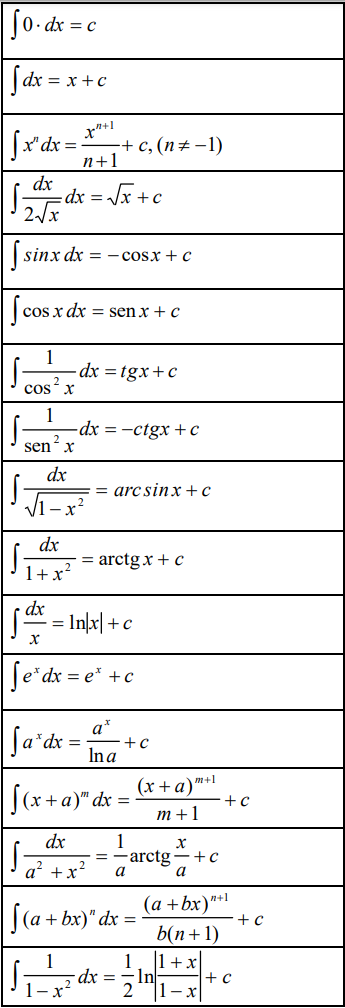
\includegraphics[scale=0.5]{integrali1.png}\\
		%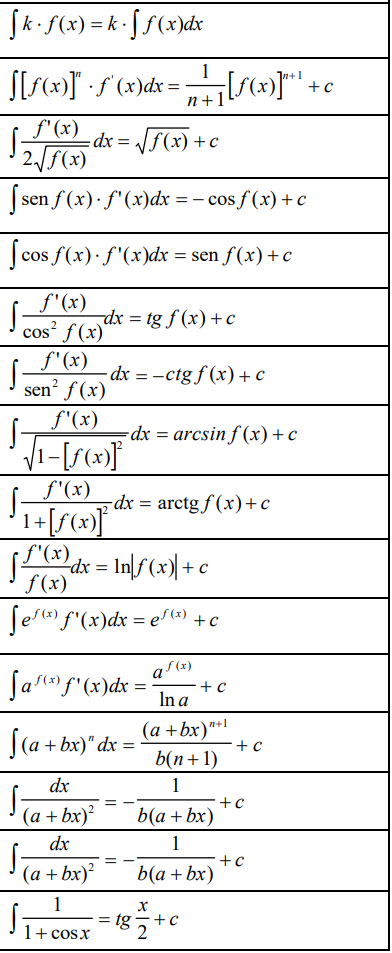
\includegraphics[scale=0.5]{integrali2.png}
		
		
		
		
		
		
		
		
		
		
		
		
		 
		
		
		
		
		
		
		
	\end{multicols*}
\end{document}